\section{Experiments}

\subsection{Datasets}


\begin{table*}[width=\textwidth,cols=6,pos=h]
\caption{Description of six selected datasets with samples for the image datasets.}\label{tbl:dataset}
\begin{tabular}{m{3cm} m{4.8cm} m{8cm}}
\toprule
Dataset name & Samples & Description \\
\midrule
COIL20
    & 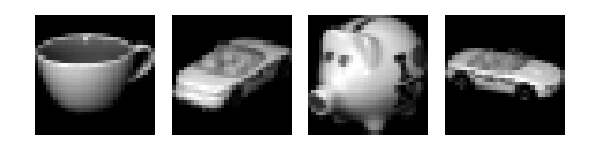
\includegraphics[width=\linewidth]{COIL20_samples}
    & 1440 grayscale images of size 32x32, belonging to 20 classes.
    The raw images of 1024 dimensions are used directly for the DR methods.\\
DIGITS
    & 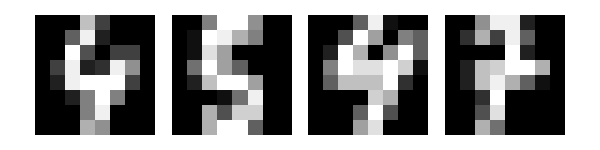
\includegraphics[width=\linewidth]{DIGITS_samples}
    & 1797 grayscale images of size 8x8 of 10 digits.
    The raw images of 64 dimensions are used directly for the DR methods.\\
FASHION\_1K
    & 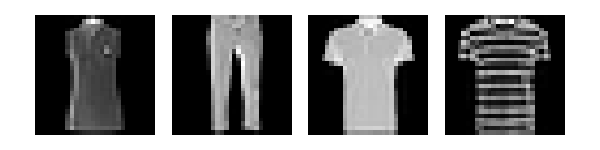
\includegraphics[width=\linewidth]{FASHION1000_samples}
    & 1000 grayscale images of size 28x28 of 10 classes, sampled from Fashion-MNIST dataset.
    The raw images of 768 dimensions are used directly for the DR methods.\\
FASHION\_MOBILENET
    & 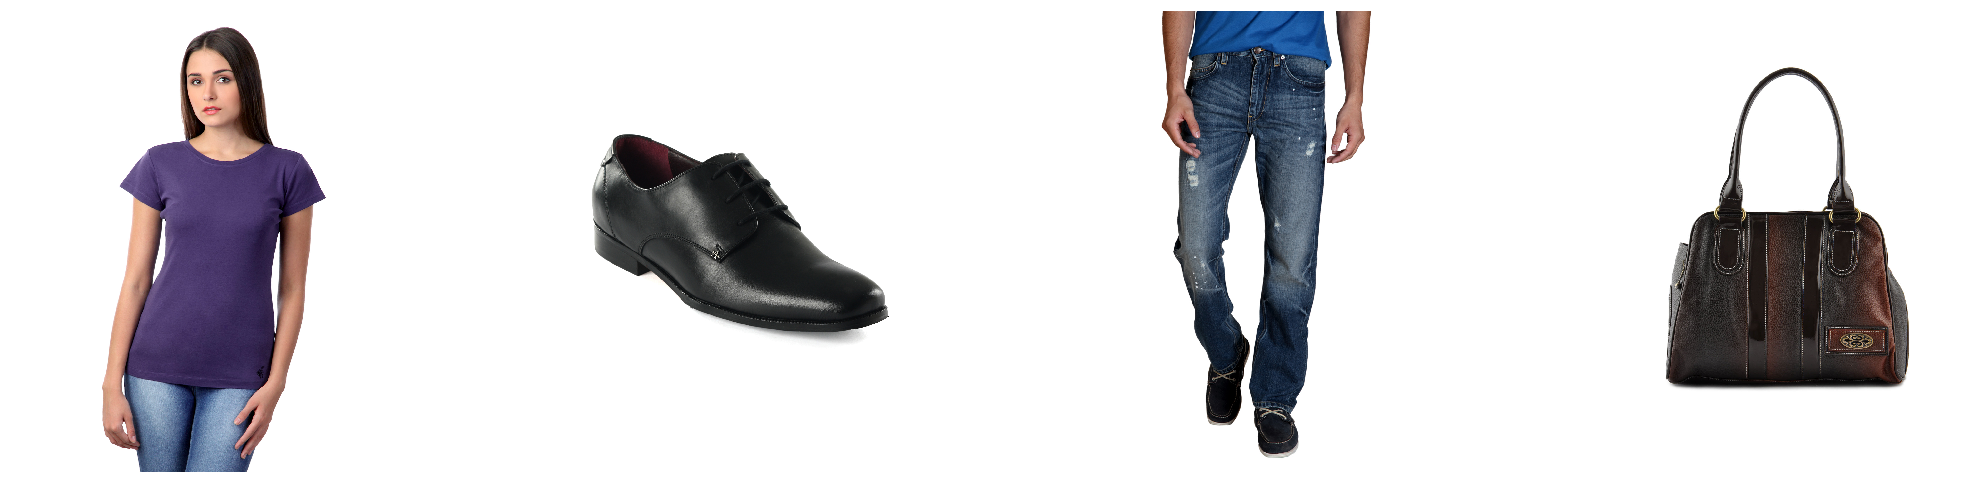
\includegraphics[width=\linewidth]{FASHION_PRODUCT_samples}
    & ??? color images of various sizes, sampled from Fashion Product images dataset.\\
5NEWS
    & 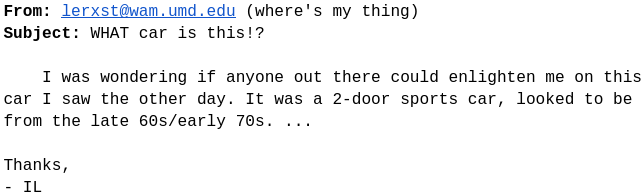
\includegraphics[width=\linewidth]{20NEWS5_samples}
    & 5 groups of 2957 emails selected from 20Newsgroups dataset, including \path{'rec.autos', 'rec.sport.baseball','sci.crypt', 'sci.space', 'comp.sys.mac.hardware'}. \\

NEURON\_1K & - & Cells from a combined cortex, hippocampus and subventricular zone of an E18 mouse \\
\bottomrule
\end{tabular}
\end{table*}


\begin{table*}[width=\textwidth,cols=6,pos=h]
\caption{This is a test caption. This is a test caption. This is a test
caption. This is a test caption.}\label{tbl1}
\begin{tabular}{m{3cm} m{4.5cm} ccc m{4.5cm}}
\toprule
Dataset name & Samples & Description \\
\midrule
COIL20
    & 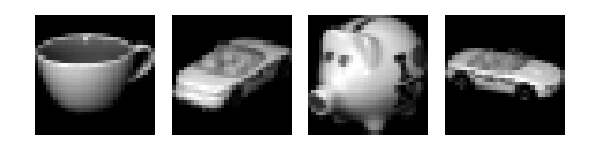
\includegraphics[width=\linewidth]{COIL20_samples}
    & 1440 grayscale images of size 32x32, belonging to 20 classes.\\
\emph{DIGITS}
    & 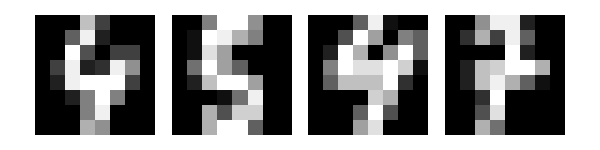
\includegraphics[width=\linewidth]{DIGITS_samples}
    & 1797 & 64 & 10\\
\emph{FASHION\_1K}
    & 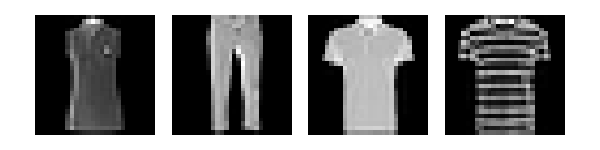
\includegraphics[width=\linewidth]{FASHION1000_samples}
    & 1000 & 784 & 10\\
FASHION\_MOBILENET
    & 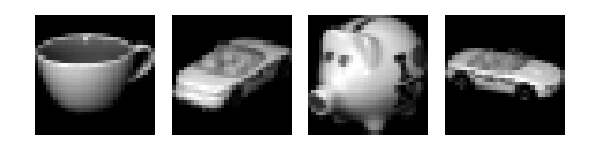
\includegraphics[width=\linewidth]{COIL20_samples}
    & - &  & - \\

5NEWSGROUPS & - & - & - \\

NEURON\_1K & - & - & - \\
\bottomrule
\end{tabular}
\end{table*}


\subsection{Constraint Generation}


\subsection{Proof of Concept}

\section{Conclusion and Future Work}

\par (1) Repeat the problem of hyperparameter tuning for DR methods and our solution:

+ The proposed constraint-based score is indenpendent to how the embedding is produced and can be used with any DR methods.
This score is built upon a limited number of constraints but can distinguish the visualizations prefering local structure and those prefereing global structure.

+ A finding that Bayesian Optimization approach fits well in our problem.


\vspace{8pt}
\par (2) Summary the advantages of the two above elements

+ The constraint-based score agree the the well-known quality metric.

+ This score can be visually represented to explain the violated pairs.

+ By combining this score with BayOpt approach, we can tune many hyperparameters at the same time for many widely used DR methods like t-SNE or UMAP.

+ BayOpt takes into account the uncertainty in the score values and also explainable. We can observe the internal optimization step to anwser the question: why to choose the next promissing hyperparameters to try?


\vspace{8pt}
\par (4) Future work:

(a) User experiment:

+ Integrate the user's feedback in two stages of our workflow.
The users can select the pairwise constraints or label some points (used to generate the constraints) to build the score.
They can also manualy select the next hyperparameters to evaluate in a customized interactive BayOpt framework.

+ Take the preference of the users on the presented visualizations to evaluate the quality of the visualization. We search for if the best visualization selected by the user corresponds to the result of our method.


(b) Integrate directly the pairwise constraints into the optimization process of BayOpt.
BayOpt is now used as a generic toolbox to find the extreme of a blackbox costly objective function.
Our idea is to use the pairwise constraint to modify the kernel in the covariance function of Gaussian Process model, which is the core element of BayOpt.
